\section{Small founding populations and competing jumps}
\label{sec:small-populations}

Criticality is an asymptotic classification.  A population founded by one or a few
individuals must first survive its early generations, and those generations remain
highly variable even on the supercritical side of the threshold.  This section
quantifies that early loss, extends the calculation to \(k\) independent founders,
and then connects the discrete process to rupture and continuous-time birth--death
mechanisms.

\subsection{Early survival and \texorpdfstring{\(k\)}{k} founders}
\label{sec:k-founders}

For a single founder, the binary recursion
\begin{equation}
  u_{n+1}=1-p+pu_n^2,
  \qquad
  S_{n+1}=2pS_n-pS_n^2
  \label{eq:early-survival-recursions}
\end{equation}
starts at \(u_0=0\) and \(S_0=1\).  At criticality the first four extinction
probabilities are
\begin{equation}
  u_1=0.500,
  \quad u_2=0.625,
  \quad u_3=0.6953125,
  \quad u_4=0.7417297\ldots.
  \label{eq:early-critical-u}
\end{equation}
Equivalently, survival through two generations has probability
\begin{equation}
  S_2=\frac12\left(1-\frac14\right)=\frac38.
  \label{eq:two-generation-survival}
\end{equation}
The factor \(1/2\) requires the founder to divide, while \(1-1/4\) requires at least
one of its two descendants to divide in the next generation.

\begin{figure}[htbp]
\centering
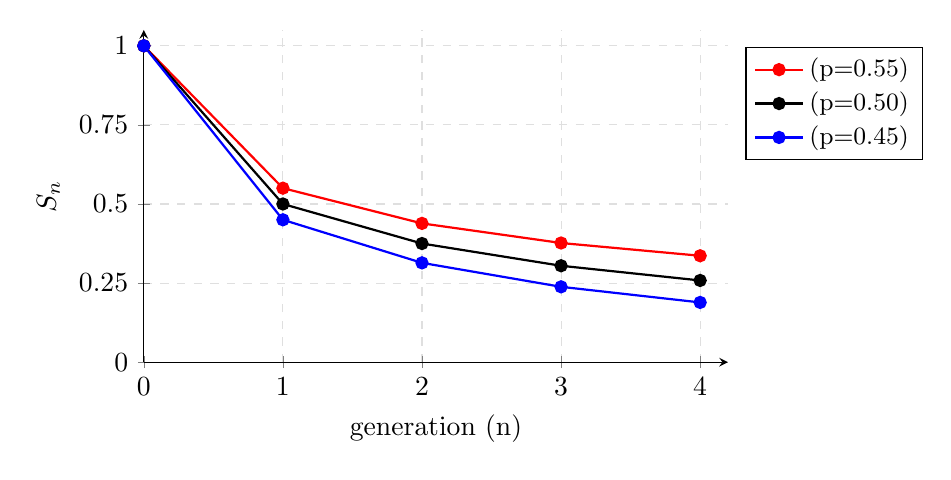
\begin{tikzpicture}
\begin{axis}[
  width=9.0cm,height=5.8cm,
  axis lines=left,xlabel={generation (n)},ylabel={$S_n$},
  xmin=0,xmax=4.2,ymin=0,ymax=1.05,
  xtick={0,1,2,3,4},ytick={0,0.25,0.5,0.75,1},
  grid=major,grid style={dashed,gray!25},
  legend style={font=\small,at={(1.03,0.95)},anchor=north west}]
  \addplot[red,thick,mark=*] coordinates
    {(0,1) (1,0.55) (2,0.438625) (3,0.3766719) (4,0.336304)};
  \addlegendentry{(p=0.55)}
  \addplot[black,thick,mark=*] coordinates
    {(0,1) (1,0.5) (2,0.375) (3,0.3046875) (4,0.2582703)};
  \addlegendentry{(p=0.50)}
  \addplot[blue,thick,mark=*] coordinates
    {(0,1) (1,0.45) (2,0.313875) (3,0.2381546) (4,0.188816)};
  \addlegendentry{(p=0.45)}
\end{axis}
\end{tikzpicture}
\caption{Survival over the first four generations from one founder.  The early
loss is steep in all three regimes; a modest supercritical advantage does not remove
the founding bottleneck.}
\label{fig:early-survival}
\end{figure}

Now let \(Z_0=k\).  The \(k\) descendant trees are independent, and each is extinct
by generation \(n\) with probability \(u_n\).  The probability that at least one
lineage remains is therefore
\begin{equation}
  S_n^{(k)}=1-u_n^k=1-(1-S_n)^k.
  \label{eq:k-founder-survival}
\end{equation}
This identity separates two effects: \(S_n\) contains the dynamics of one lineage,
whereas the exponent \(k\) contains the founding size.  For small \(S_n\),
\(S_n^{(k)}\sim kS_n\) when \(kS_n\ll1\), but the exact formula is needed once the
survival chance is no longer small.

\begin{figure}[htbp]
  \centering
  
\includegraphics[width=0.56\textwidth]{kvals.png}
  \caption{Survival probability \cref{eq:k-founder-survival} through 500
  generations at \(p=0.5\), for \(k=1,10,100,1000\).  A larger founding population
  delays extinction, but every curve still tends to zero at criticality.}
  \label{fig:k-critical}
\end{figure}

\begin{figure}[htbp]
  \centering
  \begin{subfigure}[b]{0.47\textwidth}
    \centering
    
\includegraphics[width=\textwidth]{kvals505.png}
    \caption{\(p=0.505\)}
  \end{subfigure}
  \hfill
  \begin{subfigure}[b]{0.47\textwidth}
    \centering
    
\includegraphics[width=\textwidth]{kvals495.png}
    \caption{\(p=0.495\)}
  \end{subfigure}
  \caption{The same founding sizes just above and below criticality.  The curves
  separate slowly at first and then reflect the different limiting survival laws.}
  \label{fig:k-near-critical}
\end{figure}

Conditioning an ensemble on survival also selects realisations with unusually
favourable early histories.  An apparent early excess of reproduction can therefore
arise even when every individual in every realisation obeys the same offspring law.
This is a survivorship effect rather than a change of mechanism: selection is being
performed on paths after they have been generated.  The steep early decline in
\cref{fig:early-survival} is the source of that bias.

\subsection{A discrete rupture mechanism}
\label{sec:discrete-rupture}

The binary process can be augmented by a catastrophe that ends the whole population.
The following elementary construction is retained as a bridge to the
birth--death--catastrophe models developed later in the thesis; it is not intended
as a full theory of those models.

Suppose first that the population doubles deterministically at each generation until
rupture.  Each individual present during a step independently initiates rupture with
probability \(\kappa\in[0,1]\), and a single initiation terminates the process.  The
population exposed during generations \(0,\ldots,n-1\) has total size
\begin{equation}
  1+2+\cdots+2^{n-1}=2^n-1.
\end{equation}
It follows that the probability of no rupture before generation \(n\) is
\begin{equation}
  R_n=(1-\kappa)^{2^n-1}.
  \label{eq:pure-birth-no-rupture}
\end{equation}
At step \(n\) itself, where \(2^{n-1}\) individuals are exposed, the conditional
probability of rupture is
\begin{equation}
  1-(1-\kappa)^{2^{n-1}}.
  \label{eq:rupture-at-step}
\end{equation}

When death is allowed, the accumulated exposure is random.  Let
\(\widetilde Z_i\) denote the binary Galton--Watson population with the rupture
mechanism switched off, and set
\begin{equation}
  H_n=\sum_{i=0}^{n-1}\widetilde Z_i.
  \label{eq:exposure-Hn}
\end{equation}
Conditioning on the whole catastrophe-free genealogy gives the exact identity
\begin{equation}
  \Prob(\text{no rupture before }n)
  =\E\left[(1-\kappa)^{H_n}\right].
  \label{eq:no-rupture-expectation}
\end{equation}
Since \(h\mapsto(1-\kappa)^h\) is convex, Jensen's inequality supplies the lower
bound
\begin{equation}
  \Prob(\text{no rupture before }n)
  \geq(1-\kappa)^{\E[H_n]},
  \label{eq:no-rupture-jensen}
\end{equation}
where, with \(m=2p\),
\begin{equation}
  \E[H_n]=\sum_{i=0}^{n-1}m^i
  =
  \begin{cases}
    \dfrac{1-m^n}{1-m},&m\neq1,\\[2mm]
    n,&m=1.
  \end{cases}
  \label{eq:mean-exposure}
\end{equation}
Thus replacing the random exposure by its mean is not an identity, but it does have
a precise lower-bound interpretation for the event of non-rupture.

Non-rupture should not be confused with population survival.  If the requirement is
that the population be both unruptured and non-zero at generation \(n\), then the
exact probability is
\begin{equation}
  \E\left[\ind_{\{\widetilde Z_n>0\}}(1-\kappa)^{H_n}\right],
  \label{eq:joint-survival-no-rupture}
\end{equation}
for which \cref{eq:no-rupture-jensen} does not directly provide a bound.  This
distinction removes an ambiguity in the elementary approximation and also indicates
why the joint quasi-stationary problem is better posed through the killed-chain
generator developed in later chapters.

\subsection{The linear continuous-time birth--death process}
\label{sec:continuous-bd}

Let \(X_t\in\Nzero\) have per-capita birth rate \(\lambda>0\) and death rate
\(\mu>0\).  From state \(i\geq1\),
\begin{equation}
  i\longrightarrow i+1\quad\text{at rate }i\lambda,
  \qquad
  i\longrightarrow i-1\quad\text{at rate }i\mu,
  \label{eq:linear-bd-rates}
\end{equation}
with \(0\) absorbing.  The process is the continuous-time branching analogue of
\cref{eq:binary-law}.  Its extinction law follows from the one-founder backward
equation.

\begin{proposition}[Finite-time extinction]
\label{prop:continuous-bd-extinction}
Starting from \(N\) individuals, the probability of extinction by time \(t\) is
\cite{Allen2010}
\begin{equation}
  p_0^{(N)}(t)=
  \begin{cases}
    \displaystyle
    \left[
      \frac{\mu\{1-\e^{-(\lambda-\mu)t}\}}
           {\lambda-\mu\e^{-(\lambda-\mu)t}}
    \right]^N,
      &\lambda\neq\mu,\\[4mm]
    \displaystyle
    \left(\frac{\lambda t}{1+\lambda t}\right)^N,
      &\lambda=\mu.
  \end{cases}
  \label{eq:continuous-bd-extinction}
\end{equation}
\end{proposition}

\begin{proof}
Let
\begin{equation}
  F(s,t)=\E[s^{X_t}\mid X_0=1].
\end{equation}
During an initial interval of length \(h\), one founder dies, gives birth, or
experiences no event with probabilities \(\mu h\), \(\lambda h\) and
\(1-(\lambda+\mu)h\), up to \(o(h)\).  After a birth there are two independent
descendant populations, so the branching property gives
\begin{equation}
  F(s,t+h)
  =\mu h+\lambda hF(s,t)^2
   +\{1-(\lambda+\mu)h\}F(s,t)+o(h).
\end{equation}
Hence
\begin{equation}
  \frac{\partial F}{\partial t}
  =\lambda F^2-(\lambda+\mu)F+\mu
  =\lambda(F-1)\left(F-\frac{\mu}{\lambda}\right),
  \qquad F(s,0)=s.
  \label{eq:continuous-bd-backward}
\end{equation}
The one-founder extinction probability \(q(t)=F(0,t)\) therefore solves the same
Riccati equation with \(q(0)=0\).  Separation gives, for
\(\lambda\neq\mu\),
\begin{equation}
  q(t)
  =\frac{\mu\{1-\e^{-(\lambda-\mu)t}\}}
         {\lambda-\mu\e^{-(\lambda-\mu)t}}.
\end{equation}
When \(\lambda=\mu\), the equation is
\(q'=\lambda(q-1)^2\), which gives
\begin{equation}
  q(t)=\frac{\lambda t}{1+\lambda t}.
\end{equation}
The descendant populations of \(N\) founders are independent, and all must be
extinct; thus \(p_0^{(N)}(t)=q(t)^N\), proving the result.
\end{proof}

The survival probability is \(1-p_0^{(N)}(t)\), while
\begin{equation}
  \E[X_t\mid X_0=N]=N\e^{(\lambda-\mu)t}.
  \label{eq:continuous-bd-mean}
\end{equation}
For example, differentiating \cref{eq:continuous-bd-backward} with respect to
\(s\) at \(s=1\) gives
\(M'(t)=(\lambda-\mu)M(t)\), \(M(0)=1\), and hence the displayed mean for one
founder; independence supplies the factor \(N\).

For one founder, division of \cref{eq:continuous-bd-mean} by the survival
probability gives
\begin{equation}
  \E[X_t\mid X_t>0,X_0=1]
  =\frac{\lambda\e^{(\lambda-\mu)t}-\mu}{\lambda-\mu},
  \qquad \lambda\neq\mu.
  \label{eq:continuous-bd-conditional-mean}
\end{equation}
At \(\lambda=\mu\), the corresponding exact conditional mean is
\begin{equation}
  \E[X_t\mid X_t>0,X_0=1]=1+\lambda t.
  \label{eq:continuous-bd-critical-conditional-mean}
\end{equation}
In the subcritical case \(\mu>\lambda\),
\begin{equation}
  \lim_{t\to\infty}\E[X_t\mid X_t>0]
  =\frac{\mu}{\mu-\lambda}
  =\frac{1}{A_{\mathrm c}}.
  \label{eq:continuous-qsd-mean}
\end{equation}
For fixed \(N>1\), both the mean and the late survival probability acquire the same
factor \(N\), so the limit is unchanged.  Parameterising the two competing event
types by their conditional birth probability
\begin{equation}
  p=\frac{\lambda}{\lambda+\mu}
  \label{eq:continuous-p-parameterisation}
\end{equation}
gives
\begin{equation}
  A_{\mathrm c}(p)
  =1-\frac{\lambda}{\mu}
  =\frac{1-2p}{1-p},
  \qquad 0\leq p<\frac12.
  \label{eq:Ac-definition}
\end{equation}
Unlike its discrete-time counterpart, \(A_{\mathrm c}\) is elementary.  The
comparison between \(A_{\mathrm c}(p)\) and \(A(p)\) will become exact once the
series representation of \cref{sec:A-series-bounds} is available.

\subsection{Birth--death with catastrophe as a killed chain}
\label{sec:bdc-setup}

The later birth--death--catastrophe models can be placed in a common framework
without introducing their full parameter catalogues here.  Let the positive state
\(i\) have birth rate \(\lambda_i\), ordinary death rate \(\mu_i\), and catastrophe
rate \(\kappa_i\).  A catastrophe sends the process directly to \(0\):
\begin{align}
  i&\longrightarrow i+1 &&\text{at rate }\lambda_i,
  \notag\\
  i&\longrightarrow i-1 &&\text{at rate }\mu_i,
  \notag\\
  i&\longrightarrow0   &&\text{at rate }\kappa_i.
  \label{eq:bdc-rates}
\end{align}
The jump \(1\to0\) may therefore occur through ordinary death or catastrophe.  On
bounded test functions, the generator is
\begin{multline}
  (\mathcal Lf)(i)
  =\lambda_i\{f(i+1)-f(i)\}
   +\mu_i\{f(i-1)-f(i)\}\\
   +\kappa_i\{f(0)-f(i)\},
  \qquad i\geq1,
  \label{eq:bdc-generator}
\end{multline}
with \((\mathcal Lf)(0)=0\).  Linear birth and death correspond to
\(\lambda_i=i\lambda\) and \(\mu_i=i\mu\); the catastrophe sequence can remain
general.

Restricting the generator to the positive states gives the killed subgenerator
\(K\).  Its off-diagonal entries are
\begin{equation}
  K_{i,i+1}=\lambda_i,
  \qquad
  K_{i,i-1}=\mu_i\quad(i\geq2),
\end{equation}
and
\begin{equation}
  K_{i,i}=-(\lambda_i+\mu_i+\kappa_i).
  \label{eq:bdc-subgenerator}
\end{equation}
The missing row mass is exactly the instantaneous absorption rate: it is
\(\kappa_i\) for \(i\geq2\) and \(\mu_1+\kappa_1\) for \(i=1\).  If
\(T_0=\inf\{t\geq0:X_t=0\}\), summing the positive-state forward equations gives
\begin{equation}
  \frac{\dd}{\dd t}\Prob(T_0>t)
  =
  -\mu_1\Prob(X_t=1)
  -\sum_{i\geq1}\kappa_i\Prob(X_t=i),
  \label{eq:bdc-survival-loss}
\end{equation}
where all probabilities on the right are understood before absorption.  Ordinary
death removes survival mass only from state \(1\); catastrophe can remove it from
every positive state.

This balance also sharpens the connection with quasi-stationarity.  If a
distribution \(\nu=(\nu_i)_{i\geq1}\) is quasi-stationary and the relevant sums are
finite, then for some \(\theta>0\)
\begin{equation}
  \nu K=-\theta\nu,
  \qquad
  \Prob_\nu(T_0>t)=\e^{-\theta t}.
  \label{eq:bdc-qsd-eigenrelation}
\end{equation}
Indeed, quasi-stationarity writes the unnormalised positive-state law as
\(a(t)\nu\).  The semigroup property forces \(a(s+t)=a(s)a(t)\), and
right-continuity gives \(a(t)=\e^{-\theta t}\).  Differentiating at zero yields the
left eigenvector relation.  Summing its coordinates and using
\cref{eq:bdc-survival-loss} identifies the decay rate:
\begin{equation}
  \theta
  =\mu_1\nu_1+\sum_{i\geq1}\kappa_i\nu_i.
  \label{eq:bdc-qsd-decay-rate}
\end{equation}

A constant catastrophe clock is a useful limiting case.  If
\(\kappa_i\equiv\kappa\) on the positive states, that clock may be taken independent
of the underlying birth--death process.  Its killed semigroup is
\begin{equation}
  P_t^{K}=\e^{-\kappa t}P_t^{\mathrm{BD},K}.
  \label{eq:constant-catastrophe-semigroup}
\end{equation}
The extra clock shifts the survival decay rate by \(\kappa\) but leaves the law
conditional on survival unchanged.  By contrast, a state-dependent sequence such
as \(\kappa_i=i\kappa\) weights paths according to their accumulated population
exposure and generally changes the quasi-stationary law itself.  Later chapters use
this killed-generator viewpoint; the present chapter needs only the distinction and
the eigenrelation \cref{eq:bdc-qsd-eigenrelation}.

\FloatBarrier
